\documentclass[final]{report}
\usepackage[utf8]{inputenc}
\usepackage[export]{adjustbox} 
\usepackage{pdfpages}
\usepackage{graphicx}
\usepackage{authblk}
\usepackage[danish]{babel}
\usepackage{csquotes}
\usepackage[nottoc]{tocbibind}
\addto{\captionsdanish}{\renewcommand{\abstractname}{Abstract}}
\setlength{\parindent}{4em}
\usepackage{listings}
\usepackage{minted}
\usepackage{color}
\usepackage{babel}
\definecolor{dkgreen}{rgb}{0,0.6,0}
\definecolor{gray}{rgb}{0.5,0.5,0.5}
\definecolor{mauve}{rgb}{0.58,0,0.82}

\usepackage[
    backend=biber,
    style=authoryear
]{biblatex}
\bibliography{litterature}

\lstset{frame=tb,
  language=Java,
  aboveskip=3mm,
  belowskip=3mm,
  showstringspaces=false,
  columns=flexible,
  basicstyle={\small\ttfamily},
  numbers=none,
  numberstyle=\tiny\color{gray},
  keywordstyle=\color{blue},
  commentstyle=\color{dkgreen},
  stringstyle=\color{mauve},
  breaklines=true,
  breakatwhitespace=true,
  tabsize=3
}

\usepackage[
top    = 2.75cm,
bottom = 2.75cm,
left   = 3.00cm,
right  = 3.00cm]{geometry}

\usepackage{fancyhdr}
\pagestyle{fancy}

\begin{document}
\begin{titlepage}
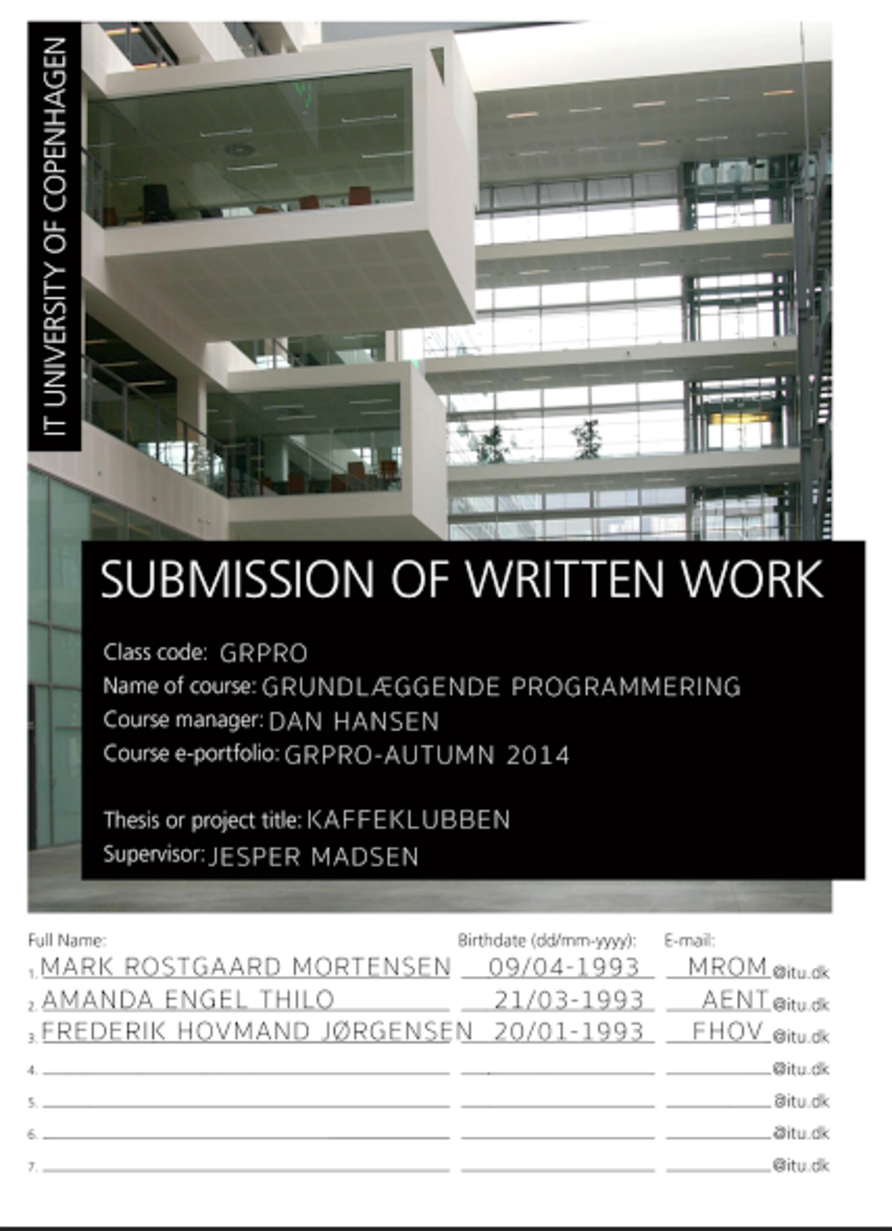
\includepdf{frontpage.pdf}
\end{titlepage}



\includepdf[width=400pt]{forside.pdf}



 
\baselineskip= 15pt

\title{Forord}
Denne rapport er udarbejdet i December 2014 i et fire ugers projekt på IT-Universitetet i København under vejledning af Jesper Madsen.
I projektet udviklede vi et softwaresystem til booking i biografer skrevet i Java. Programmet har til opgave at skulle assisterer en ekspedient i personens arbejdsopgaver der har med kundehenveldelser af gøre, f.eks: Book nye pladser eller slette en tidligere bestilling. Programmet skal ikke kunne håndtere salg.

\tableofcontents

\chapter{Indledning}
\section{Baggrund}
Det problemområde vi har arbejdet med i forbindelse med vores projekt, er udviklingen af et softwaresystem til brug for en ekspedient der betjener en billetluge i en biograf. Det område der skulle dækkes var reservation både når kunden stod foran billetlugen, samt når kunden ringede ind på telefon. Vores løsning skulle håndtere   ekspedientens arbejdsopgaver i sådanne situationer. Løsningen skal derfor fokusere udelukkende på reservationer, og ikke salg. 

\section{Problemstilling}
Den overordnede problemstilling som vores program besvarer, er hvordan man udvikler et simpelt, brugervenligt og databasebaseret softwaresystem til brug for en ekspedient i en mindre biografs billetluge. 

\subsection{Krav til programmet}
Af krav til programmet [\cite{opg}] kan nævnes at der i forbindelse med reservationerne skal oplyses navn eller anden identitet på kunden. Vi har i vores program valgt at den centrale information omkring brugeren er dennes telefonnummer. Det har vi gjort af den grund af flere kunder godt kan have samme navn, men at ens telefonnummer er unikt.  

Derudover skal biografen indeholde flere sale, og sende flere forskellige forestillinger i løbet af dagen. Salenes størrelse, antal pladser mm. skal fremgå af databasen frem for at være indkodet i selve programteksten. Derfor har vi i stedet for at skrive data ind i programteksten, valgt at lave en speciel klasse til at hente data fra databasen. Det samme er gældende for de enkelte forestillinger, der derfor også bliver gemt i databasen.
\\
\\
Kravene er oplistet nedenfor

\begin{itemize}
\item Reserverings process

\begin{itemize}
\item vælge forestillinger, herunder dato, tid, film og sal
\item vælge pladser
\item vise optaget og ikke optaget pladser
\item bestille pladser
\item afbestille pladser
\item vis ''Dine sæder''
\end{itemize}

\item Kigge process
\begin{itemize}
\item se film der går
\item se tider

\end{itemize}
\end{itemize}

\subsection{Brugerscenario}
Signe er ekspedient i en mindre biograf og bruger \emph{biobooking} til at reserverer biletter til kunder. Hun tænder systemet når hun møder på arbejde. Dagens første kunde optræder lidt over kl. 10. Kunden ønsker at booke tre billetter til Fury kl 17.30 den 19. Januar 2015. Signe klikker på den filmknap hvordpå navnet\emph{Fury} optræder. Herefter klikker hun på knappen med tiden \emph{17.30} som står under datoen \emph{19/1}. Signe spørger nu kunden hvor i salen kunden ønsker sine pladser. Kunden siger \emph{ca. midt i salen}. Signe vælger sæde \emph{9, 10 og 11} på række \emph{F}, og viser det på skærmen til kunden. Kunden er tilfreds, så Signe spørger kunde om hvilket navn og telefonnumer reservationen skal laves i. Efter at have indtastet kundens informationer klikker Signe på \emph{Fuldfør reservation}. Kunden tager hjem og opdager, at der er kommet en tilmelding mere til biografturen hun tidligere bookede billetter til. Derfor ringer vedkommende ind til biografen og får fat på ekspedienten Signe. Signe klikker på \emph{Ret reservation} og indtaster kundens telefonnummer. Signe får nu vist en liste med alle reservationer for det pågældende nummer til forestillinger som endnu ikke har været vist. Derefter vælger Signe den pågældende reservation som skal redigeres. Kunden fortæller Signe, at der kommer en ekstra deltager til arrangementet, så de skal have et sæde mere tilføjet til reservationen - de bliver altså fire personer i stedet for tre. Signe kan se de allerede valgte sæder markeret med blå og kan desuden se, at sædet til højre for de reserverede sæder er reserveret til en anden kunde. Heldigvis er der ledigt til venstre, så der klikker Signe og tilføjer derved et ekstra sæde til reservationen. Nu er der fire blå sæder og Signe afslutter redigeringen ved at klikke på \emph{Rediger reservation}. Så er reservationen rettet og kunden er tilfreds med den service vedkommende har fået.

\subsection{Systemdesign}
Vores system er overordnet baseret på data fra databasen. Systemet generer layout ud fra forskellige data i databasen. Dette indebærer bl.a. hvilke film der er i film-tabellen, hvilke forestillinger der er tilknyttet til en given film, hvilke reservationer der er tilknyttet en given forestilling, hvilke reservationer der er tilknyttet et givent telefonnummer mv. Programmet er delt op, så mest mulig databehandling foretages hos klienten/brugeren. Dette indebærer objekter med informationer om de forskellige forestillinger, arrays med valgte sæder mv. Databaseforespørgsler er lavet så omfattende som muligt, så der udføres så få forespørgsler som muligt og data gemmes i objekter og arrays eller bliver benyttet med det samme i den grafiske fremstilling af programmet som eksempelvis ved generering af film-knapper. 


\chapter{Problemanalyse}

\section{Vores løsning}
Den overordnede problemstilling vi har valgt at fokusere på, er hvordan man udvikler et simpelt og implicit program der både og brugervenligt og hvor databasen opbevarer det meste data. 

Vores program løser problemstilligen ved at have alt information omkring forestillinger, sale, film og reservationer gemt i en database. Dette gør selve koden og databasen nem at vedligeholde, og vi har på den måde undgået unødvendig kodeduplikering [\cite{GRPRO8}]. For at opfylde ønsket om brugervenlighed har vi valgt at vise programmet i ét vindue, hvor brugeren nemt kan navigere, ved hjælp af tabs, imellem de forskellige funktionaliteter programmet har.

\subsection{Build Reservation}
En af de større udfordringer, som man også har kunne tackle på en masse forskellige måder, var når biografsalen skulle bygges op rent grafisk. Den primære metode vi brugte her var \emph{buildReservationScene(int showID)} i vores \emph{controller.java} class. Alt informationen omkring biografsalen får vi fra vores database, dette bliver behandlet i metoden, her er det bl.a. de forskellige labels der bliver sat (cinemaNameLabel, movienameLabel etc.) Med informationen fra databasen kører vi et for-loop der kører igennem rækkerne, og inden i for loopet kører der endnu et for-loop der kører sæderne igennem for hver kolonne. Det er rimelig lige til og i højgrad den bedste måde vi kunne komme på at gøre det. Koden nedenfor viser hvordan det er lavet. 

\begin{minted}{java}
for(number of rows){
    for(number of collums){
        if(seats are reservated){
            make seats red
        } else {
            make seats green
        }
    }
}
\end{minted}

Sæderne bliver grafisk vist som firkanter, her kunne man godt have lavet det som knapper. Vi valgte at bruge rectangle objekter fordi det var nemt at manipulere det udseende vi gerne ville give dem uden at vi behøvede at gå på kompromis med funktionaliteten.

Til sidst er der måden hvorved du reserverer flere pladser. En oplagt mulighed ville være at have en dropdown menu i bunden af vinduet, der, når den klikkes, viser en liste fra med tal fra 1 til antallet af frie sæder (hvis der er nogle frie sæder tilbage). Denne mulighed er ganske fin, vi besluttede os dog for at gå med noget mere interaktivt hvor ekspedienten blot skal trække musen henover de sæder der skal vælges for at vælge dem. Dette er en feature der gør det nemmere for ekspedienten at vælge en masse sæder på engang og samtidig super fleksibelt, hvis en reservation eksempelvis skal deles op på flere rækker. 

\subsection{Alternative løsninger}
En alternativ måde at løse problemstillingen på ville være at fokusere på andre måder at booke billetter på. Vi har valgt at man først skal vælge film, derefter tid og tilsidst sæder. Man kunne have valgt at gøre det muligt for brugeren at vælge dato eller tid før valg af film. Vi har dog valgt den løsning vi syntes var mest brugervenlig. En anden mulighed er at man kunne have lavet en liste der viste \emph{alle} forestillinger sorteret efter spilletid - uden at tage hensyn til sortering i forhold til film. Denne mulighed syntes vi designmæssigt ville fungere meget rodet og ikke intuitiv på nogen måde. Derudover kunne vi have valgt at gemme vores reservationer i programkoden frem for i databasen. Vi diskuterede dette i begyndelsen af projektet, men fandt det for besværligt at arbejde med, da det ville kræve større mængder kode, fylde mere plads samt resultere i at vores program formentlig ville bruge længere tid på at compille og køre. Derudover er det langt mere hensigtsmæssigt at vedligeholde og rette data sådom reservationer i en database fremfor i en evt. teksfil. Desuden ville en tekstfil med reservationer eller anden programdata kræve forskellige rettigheder affængig af operativsystemmet. Dette problem er slet ikke aktuelt i vores løsning, da alt sammen ligger i databasen. 

\section{Databasedesign}
En af de to overordnede tabeller i vores database er \emph{cinemas} som indeholder information omkring vores biografsale. Dette omfatter salens navn, id, antal rækker og antal sæder i hver række. Vores sæder er ikke repræsenteret som en tabel i vores database, men derimod gemt som et 2 dimentionelt array. 

Den anden vigtige tabel er \emph{movies} som indeholder information omkring de film der går i biografen. Det eneste inforamtion denne tabel holder er navn og id. I begge tabeller er det, det pågældende id som fungerer som nøgle. Altså sal\_id og movie\_id.  

De to tabeller \emph{movie} og \emph{cinema} bliver koblet sammen i tabellen \emph{show}. Her bruges deres nøgler til at sammensætte de foreskellige forestillinger som vores biograf kan vise. I \emph{shows} tilføjes så et nyt ide til de enkelte forestillinger samt et timestamp - som er det tidspunkt forestillingen skal begynde.


\chapter{Brugervejledning}
\section{Programmet}
Programmet er designet med 3 tabs i toppen. \emph{Forestillinger, Reservation og Ret reservation}. Når programmet åbnes starter brugeren i \emph{Forestillinger-vinduet} og der vises en liste i venstre side med de film som kører i biografen. Brugeren klikker på den film, som kunden ønsker at reservere billetter til. Når en film vælges bliver tiderne for filmforestillinger vist for den pågældende film. \\


\begin{figure}[h]
\centering
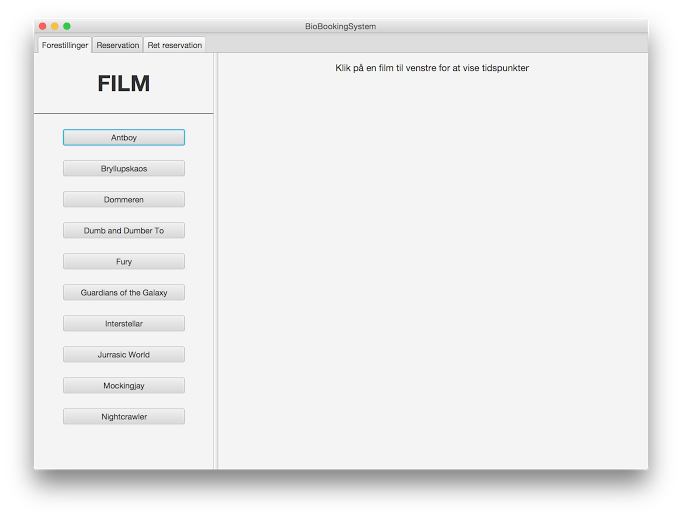
\includegraphics[width=200pt]{1.png}
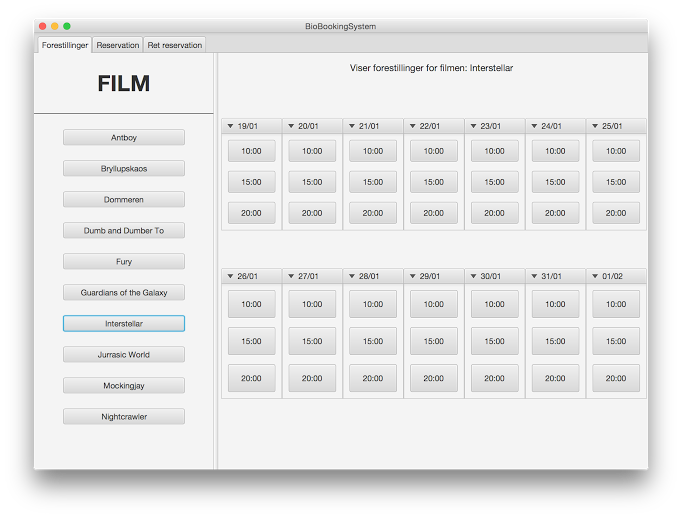
\includegraphics[width=200pt]{2.png}
\caption{Forestillinger-vinduet før og efter en film er valgt}
\end{figure}



Klikker ekspedienten derimod ikke på noget, vil der stå følgene tekst \emph{Klik på en film til venstre for at vise tidspunkter}, og har man ikke først valgt film og tidspunkt vil \emph{Reservation} være ubrugelige.

Efter at have valgt film, vælger brugeren tidspunktet, som kunden ønsker at reservere til. Når en forestilling vælges bliver brugeren videreført til næste tab - altså reservation. Her vises et vindue med firkanter som illustrerer sæderne i biografen. Ledige sæder er illustreret som en grøn firkant og optagede sæder er illustreret som røde sæder. Brugeren klikker på de sæder som kunden ønsker at reservere - brugeren kan desuden holde musen nede og hive musen over de sæder som skal vælges. De valgte sæder skifter farve til blå og brugeren kan se hvor mange sæder vedkommende har markeret nederst i venstre hjørne. 

\begin{figure}[h]
    \centering
    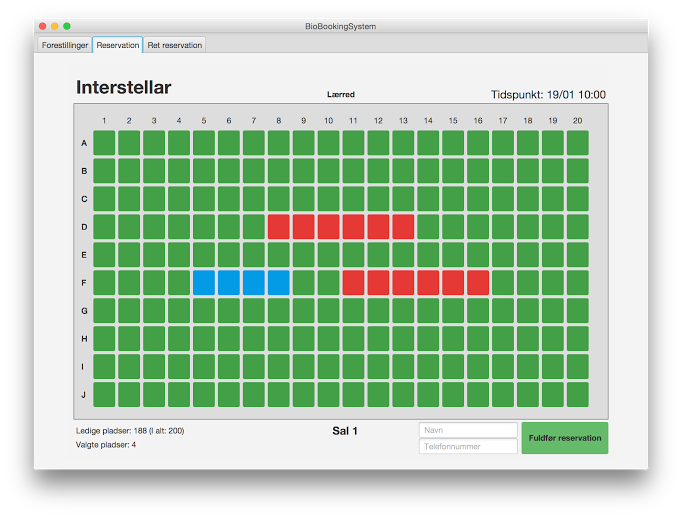
\includegraphics[width=250pt]{3.png}
    \caption{Biograf sal med reserverede og valgte sæder}
\end{figure}

Når sæderne er valgt skrives kundens navn og telefonnummer ind i tekstfelterne nederst i højre hjørne. Afslutningsvist trykkes der på knappen \emph{Fuldfør reservation}. 

Hvis kunden fortryder sin bestilling eller har ændringer til en eksisterende bestilling, så klikker brugeren på tabben \emph{Ret reservation} i toppen af programmet. Brugeren bliver taget til et vindue hvor kundens telefonnummer skal indtastes. Når telefonnummeret er indtastet og der er trykket på Enter-tasten eller på \emph{Tjek reservationer}-knappen, så vises en liste nedenunder med de reservationer som kunden har tilknyttet til sit telefonnummer. Der vises kun reservationer for forestillinger som ikke er blevet vist - gamle reservationer vises altså ikke. Brugeren dobbeltklikker på den reservation der skal rettes og et nyt vindue åbner som ligner reservationsvinduet. De optagede sæder er røde, de ledige er grønne og de sæder som er tilknyttet til den pågældende reservation vises som blå. Brugeren kan tilføje eller slette sæder. Et valgt sæde er blåt og markeringen fjernes ved at klikke på sædet igen. Når ændringen til reservationen er valgt, så klikker brugeren på \emph{Rediger reservation}. Skal reservationen derimod slettes helt, så klikker brugeren på \emph{Slet reservation}.

Hvis kunden fortryder sin bestilling eller har ændringer til en eksisterende bestilling, så klikker brugeren på tabben \emph{Ret reservation} i toppen af programmet. Brugeren bliver taget til et vindue hvor kundens telefonnummer skal indtastes. Når telefonnummeret er indtastet og der er trykket på Enter-tasten eller på \emph{Tjek reservationer}-knappen, så vises en liste nedenunder med de reservationer som kunden har tilknyttet til sit telefonnummer. \clearpage
\begin{figure}[h]
\centering
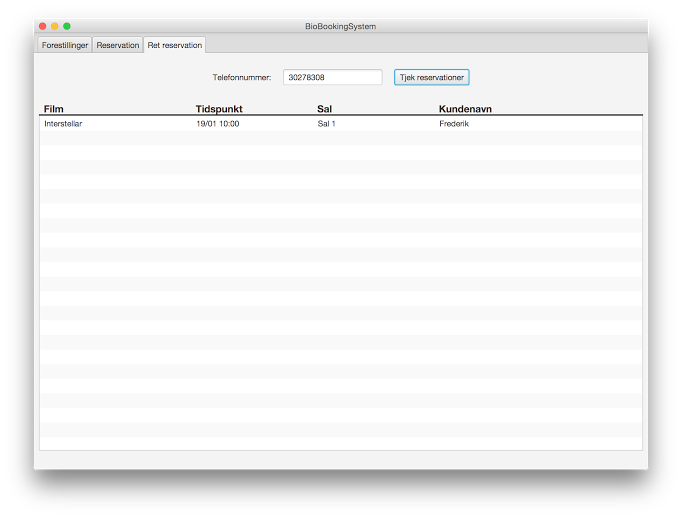
\includegraphics[width=250pt]{4.png}
\caption{Forestillinger-vinduet før og efter en film er valgt}
\end{figure}


Der vises kun reservationer for forestillinger som ikke er blevet vist - gamle reservationer vises altså ikke. Brugeren dobbeltklikker på den reservation der skal rettes og et nyt vindue åbner som ligner reservationsvinduet. \\

\begin{figure}[h]
\centering
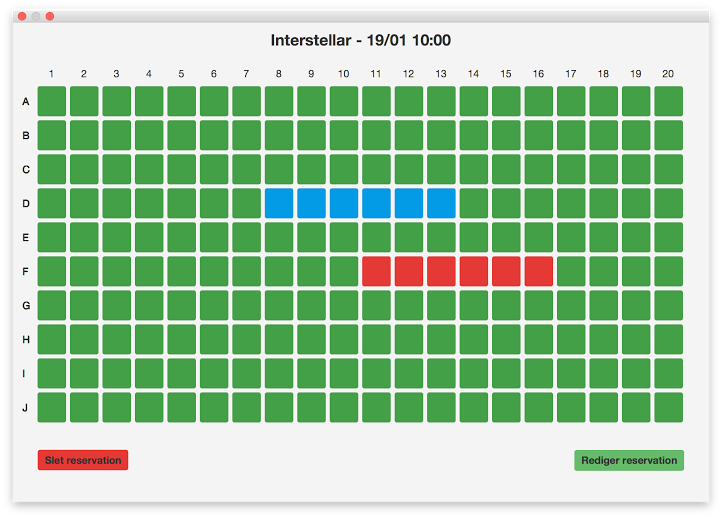
\includegraphics[width=250pt]{5.png}
\caption{Vinduet hvor brugeren retter sin reservation}
\end{figure}

De optagede sæder er røde, de ledige er grønne og de sæder som er tilknyttet til den pågældende reservation vises som blå. Brugeren kan tilføje eller slette sæder. Et valgt er blåt og markeringen fjernes ved at klikke på sædet igen. Når ændringen til reservationen er valgt, så klikker brugeren på \emph{Rediger reservation}. Skal reservationen derimod slettes helt, så klikker brugeren på \emph{Slet reservation}.

\chapter{Teknisk Analyse}
\section{Model View Controller}
Vi har brugt Model-View-Controller (fork. MVC) til at adskille vores database og buildholder (model), vores controller og vores JavaFx brugergrænseflade (view) fra hinanden. Dette gør vores programkode mere overskuelig og nemmere at vedligeholde.

\subsection{Moduler}
Programmet har 2 klasser: DBConnect og buildHolder.
DBConnect foretager alt der har med databasen at gøre. Dette er eksempelvis databaseforespørgsler hvor alle film returneres i et LinkedHashMap, hvor data såsom reservationer, salstørrelse mv. for en given forestilling hentes, hvor data såsom reservationer indsættes eller opdateres i databasen. Den væsentligste del af DBConnect-klassen må være funktionen getCon, der sørger for at der er en gyldig forbindelse til databasen. 

\begin{minted}{java}
public Connection getCon() throws SQLException {
        if(!con.isValid(30)) { // isValid takes seconds to wait for timeout as parameter
            con = DriverManager.getConnection(host, username, password);
        }

        return con;
    }
\end{minted}

En anden klasse er \emph{buildHolder}. Et \emph{buildHolder}-objekt lagrer data for en given forestilling. Der bruges getters og setters, så de data der lagres også kan hentes efterfølgende. \emph{buildHolder} objektet bruges efterfølgende til at bygge reservationssalen med data som filmnavn, tidspunkt for forestillingen, størrelsen på salen (rows/columns), reserverede sæder mv. 

Det er \emph{controlleren} der gør brug af disse objekter, når data skal visualiseres og altså fremvises for brugeren.

\subsection{Algoritmer}
Når et DBConnect objekt initialiseres bliver der oprettet og gemt en connection til databasen i et felt. Funktionen \emph{getCon} tester om denne forbindelse stadig er gyldig. Hvis den ikke er gyldig, så oprettes der en ny gyldig forbindelse og denne returneres. Derved kan forbindelsen eksempelvis kaldes som \emph{getCon().createStatement();} og altid bruge en gyldig forbindelse. \emph{getMovies} tager ingen parametre og returnerer et LinkedHashMap med filmens id som key og filmens navn som value. Sorteret alfabetisk efter filmnavn (A-Z).

\emph{getMovieSchedule} tager film id som parameter og returnerer et LinkedHashMap med show id som \emph{key} og tidspunktet for forestillingen (timestamp) som \emph{value}. Data er hentet fra databasen med en sql-query hvor film id’et er det ene \emph{where}-parameter og tiden for forestillingen er større/senere end det nuværende tidspunkt. Hele forespørgslen er sorteret med den nærmeste forestilling først - altså \emph{time} ASC. 

\emph{getBuildSceneInfo} tager et forestillings id som parameter og laver et \emph{buildHolder} objekt med information om forestillingen. Først hentes generel information såsom filmnavn, tidspunkt for forestillingen, størrelsen på salen (højde og bredde) m.fl. Efterfølgende hentes alle de reserverede sæder til den pågældende forestilling. Disse reservationer gemmes i et multidimensional array \emph{[x][y]} af typen \emph{Boolean}, hvor værdien i det ydre array er x-koordinaten til sædet og værdien i det indre array er y-koordinaten. Et reserveret sæde sættes til at være \emph{true} på sædets plads - eksempelvis vil sæde 5:7 være \emph{[5][7] = true}, hvis det er reserveret. 

\emph{insertReservation} er den metode, som sørger for at de valgte sæder og tilknyttede kundeinformationer indsættes i databasen. Der tages fire parametre: en \emph{ArrayList} af typen string med sæderne, en \emph{Integer} med forestillingens id, en \emph{String} med kundens navn og ligeledes en med kundens telefonnummer. Sæderne gemmes som string med et kolon som splitter mellem sædets \emph{x-} og \emph{y-værdi} fx 5:8.

Først indsættes kundens navn, telefonnummer og forestillingens id i tabellen \emph{reservations}. Derefter køres funktionen \emph{getLastReservationId}, som returnerer senest indsatte reservations id. Dette id skal nemlig bruges til at linke de valgte sæder med reservationen. Dernæst løbes vores \emph{ArrayList} igennem for at indsætte hvert sæde i reservation ind i vores database. \\
\begin{minted}{java}
for(String seat : seats) {
    query = "INSERT INTO reservationlines (reservation_id, seat_x, seat_y) VALUES ('"
     + lastid + "', '" + seatInfo[0] + "', '" + seatInfo[1] + "')";
  
}
\end{minted}

Koden ovenfor illustrerer hvordan vi indsætter seat i databasen. Vores sæde-string skal splittes op, så vi kan indsætte en x-værdi og en y-værdi i databasen. Man splitter vores string op i et \emph{string-array} hvor index 0 er alt tekst før første kolon. Index 1 er alt tekst før andet kolon osv.

\begin{minted}{java}
String[] seatInfo = seat.split(":");
\end{minted}

Derved kan vi nu tilgå vores x-værdi som \emph{seatInfo[0]} og vores y-værdi som \emph{seatInfo[1]}. Hvis hele metoden forløber fejlfrit, så returneres der boolean true. Hvis der forekommer en \emph{exception} så returneres false. 

\emph{getReservations} henter alle reservationer tilhørende et telefonnummer. Parametret er altså et telefonnummer og metoden returnerer et LinkedHashMap med reservations id som \emph{key} og en \emph{HBox} med informationer om forestillingen som \emph{value}. Databaseforespørgslen henter kun fremtidige reservationer - altså reservationer til forestillinger som endnu ikke er vist. Denne metode bliver brugt til at liste alle fremtidige reservationer op for en kunde, så de enten kan rettes eller slettes. 

\emph{getResSeat} bruges til at bygge den sal, hvor en reservation kan rettes eller slettes. Den tager to parametre. Det ene er reservations id’et og det andet er et buildHolder objekt. Reservations id’et er essentielt, da de reserverede sæder er bundet op på dette. BuildHolder objektet bruges til at bygge det multidimensionelle array som returneres, da vi skal bruge salens bredde og højde (columns/rows).

\begin{minted}{java}
Boolean[][] resSeat = new
Boolean[bh.getColumns()+1][bh.getRows()+1];
\end{minted}

Vi ligger 1 til, da sæderne starter med 1 og et array starter med index 0. På den måde undgår vi en \emph{NullPointerException}, da salen ellers vil prøve et tilgå et felt uden for vores array - også kaldet \emph{ArrayIndexOutOfBoundsException}. 
Et optaget sæde vil returnere værdien true og et ledigt sæde false. Dette tjekker vi når vi looper igennem salens højde og bredde, som bliver gjort i vores controller, der også bygger den grafiske sal som er det vi ser. 

\emph{getShowIdFromResId} er en forholdsvis simpel metode. Den tager et reservations id som parameter og laver ud fra dette en database forespørgsel og finder derved ud af hvilken forestilling det pågældende reservations id tilhører. Dette forestillings id returneres som en int. På den måde kan vi sætte et buildHolder objekt op med det rette informationer, når en forestilling skal redigeres eller slettes. Metoden returnerer 0 hvis der ikke er fundet nogen forestilling til det pågældende reservations id. 

\emph{updateReservation} opdaterer en reservation. Der tages tre parametre: to \emph{ArrayLists} af typen \emph{String} og et reservations id af typen \emph{int}. Den første arrayliste er de gamle reserverede sæder og den anden arrayliste er de nye reserverede sæder. Først slettes de gamle sæder og derefter indsættes sæderne fra den redigerede og dermed nye reservation. Hvis opdateringen af reservationen forløber uden fejl, så returnerer metoden \emph{true} ellers returnerer metoden \emph{false}. 

\emph{deleteReservation} sletter en reservation og dertilhørende sæder fra databasen. Metoden har et parameter som er reservations id af typen \emph{int}. Da sæderne står er linket til dette reservations id, kan vi bare fjerne alle rækkerne i tabellen med reserverede sæder ud fra et givent reservations id. Først fjernes reserverede sæder og afslutningsvist fjernes selve ordren med kundenavn, telefonnummer og forestillings id. 



\section{Design af Brugergrænseflade}
Vi har valgt at opdele vores brugergrænseflade i tre dele: \emph{Forestillinger, Reservation og Ret Reservation}. Vi diskuterede om det var mest brugervenligt at lave et vindue som skiftede mellem forskellige sider når man klikkede \emph{næste side}, men blev enig om at det var mere simpelt og brugervenligt at lave et vindue med mulighed for mauelt at skifte mellem siderne via. en \emph{tap-menu}. Siden \emph{Forestillinger} er desuden også delt op i to dele - en del der oplister de forskellige film, og en der oplister spilletiderne for den valgte film. Vi har valgt det på den måde, fordi vi syntes det var designmæssigt bedre at udfylde hele vinduet ved at opdele det i de to dele, frem for at have en stor næsten tom side. 
En anden beslutning vi diskuterede omkring vores design, var hvorvidt man skulle kunne klikke på \emph{Reservation} uden først at have valgt en forestilling. Vi havde overvejet at have en default biografsal til hvis man ikke havde valgt forestilling, men besluttede at den løsning vi har nu, hvor der blot står \emph{Du har ikke valgt nogen forestilling! Klik "Forestillinger" og vælg en film}, var mere brugervenlig. 
Under \emph{Reservation} diskuterede vi hvorvidt rækker og sæder skulle have navne, og valgte at kalde rækkerne ved bogstaver og sæderne ved tal. At man både kan klikke på de enkelte sæder \emph{og} trække hen over dem for at vælge sæder, er et resultat af at vi både ønskede at man skulle kunne vælge mange sæder på én gang, men også at man skulle kunne vælge sæderne til eller fra enkeltvis. Vi snakkede om at det skulle laves således at brugeren indtastede det ønskede antal sæder, og når brugeren så klikkede på ét sæde, ville det resterende antal sæder brugeren ønskede, automatisk blive valgt i form af de efterfølgende sæder. Vi valgte dog denne løsning fra, da vi syntes vores løsning var mere flexibel. 
Vores \emph{View} er kun én klasse, nemlig \emph{Controller}. Det er et bevidst valg vi har taget, og diskuteret. Vi besluttede os for at holde os til en klasse for enkelthedens skyld. Normalt ville man inddele \emph{View} i flere klasser med hver deres funktion. Fx. kunne vi have tre \emph{View}-klasser, en for \emph{Forestillinger}, en for \emph{Resrvation} og en for \emph{Ret reservation}. Vi syntes dog ikke det var et problem at samle dem i én klasse pga programmets størrelse. Vi har således, for vores egen forståelses skyld, valgt at gøre det i én klasse.

\subsection{Begrænsninger}
Systemet er ikke begrænset til små biografer og kan derfor også bruges af større biografer med store sale. Systemet har ikke en administration til forestillinger og betalling, men det kan implementeres rimelig simpelt i den nuværende kode, da systemet er lavet så dynamisk som muligt. Systemet baserer nemlig alt indhold i programmet fra databasen, pånær de statiske elementer som textfields og almindelige buttons. Man kan forestille sig, at systemet ville være svært at benytte for en biograf med over 3000 sæder, da sæderne i salene vil blive utroligt små og svære at markere. Som biografen er opbygget nu kan salene ikke være større end 25 rækker, medmindre man navngiver dem efter noget andet end alfabetet. Vores system er udviklet til mindre biografer og håndterer fint sale på op til 1000 sæder - dog skal man være god med museføringen, når vi har med så mange sæder at gøre, da størrelsen på sæderne skalerer til en statisk scene.

\subsection{Fejlmeddelelser}
Programmet viser exceptions ved hjælp af metoden catchPopUp, som gør brug af vores dialog boks newPopUp der tager en string som skal vises i dialogvinduet. Metoden til at vise fejlmeddelelser tager en exception som parameter og denne exception fremvises i dialogen. Systemets catchPopUp vises altid teksten “Der er opstået en fejl” efterfulgt af den pågældende exception. newPopUp-metoden derimod bruges direkte, når beskeder skal printes til brugeren. Dette indebærer beskeder som “Bestllingen er gennemført”, “Reservationen kan ikke udføres. Felterne navn og telefonnummer skal være udfyldt. Desuden skal du vælge sæder”, “Reservationen er rettet!” m.fl. Når en reservation opdateres eller indsættes returnerer metoden til dette en Boolean. Hvis den returnerer false bliver en dialog vist med enten \emph{“Der er sket en fejl. Prøv igen.”, “Der er sket en fejl! Reservationen kunne ikke rettes. Luk vinduet og prøv igen.”}. 

\chapter{Afprøvning}

\section{Brugerafprøvning}
Vi har valgt at lave vores testing af programmets JavaFx-baserede brugergrænseflade som manuel brugerafprøvning. Den beskrevne fremgangsmåde i brugervejledningen er den tilsigtede måde brugeren skal forstå og bruge programmet.
Brugeren havde ingen problemer med at reservere en forestilling, og det tog heler lang tid før brugeren havde fundet ud af at rette eller slette i reservationen. Vores bruger prøvede at indtaste bogstaver istedet for sit telefonnummer, men vores system reagerede som forventet på fejlen og et popup-vindue med en fejlmeddelelse dukkede frem. Den eneste uoverenstemmelse med hvad vi havde forventet, var at brugeren ikke opdagede at man kunne trække musen hen over sæderne for at markere flere sæder.  

\section{Unit test}
Vores klasse \emph{DBConnectTest} er en testklasse og indeholdende derfor udelukkende tests. Den primære funktion for for disse test er at teste om vores programtekst snakker rigtigt sammen med databasen. vi har oprettet en testdatabase, som indeholder de samme tabeller som vores oprindelige database. Testdatabasens tabeller er dog tomme, og bruges kun til test. 
Fordi vi primært tester koden i relation til databasen er det ikke rene unit test vi udfører. Faktisk er det det man kalder integration tests. Integration test er tests der bruger en database, et netwærk eller et andet eksternt system som fx en mailserver. Typisk for en integration test er også at den udfører I/O. I vores tilfælde tager vores tests input fra en database og udskriver et grafisk output til skærmen. \linebreak

Testen \emph{testGetMovies()} tester om film og ide passer sammen. Dette gøres ved at vi giver testen et forventet output, som er bestemte id's tilknyttet bestemte film. Når testen kører, testes derfor om det forventede output passer overens med det faktiske uddata. 

\emph{testTimeStamp()} tjekker hvorvidt en given films forestillinger bliver sorteret korrekt efter tid. Det gøres ved at lave et while-loop som kører igennem alle tidspunkterne og tjekker om det nuværende timestamp er lavere end det foregående.

For at tjekke om et reserveret sæde vise med rød farve, og dermed ikke har nogle funktioner. Sædernes funktioner er nemlig tilknyttet deres farve, således at de røde sæder ikke er mulige er klikke på. \emph{testReservedSetColor()} henter et reserveret sæde og derefter sætter dens farve ligmed den forventede røde farve. 

\emph{testInsertReservation()} tester om metoden \emph{InsertReservation()} rent faktisk opretter en reservation. \\
\begin{minted}{java}
 @Test
    public void testInsertReservation(){
        ArrayList<String> seats = new ArrayList<String>();
        seats.add("1:2");
        dbConnect.insertReservation(seats, 120, "Amanda", "26802103");
        dbConnect.getLastReservationId();
\end{minted}
 
Ovenfor ses en del af testmetoden \emph{testInsertReservation}. I metoden begynder vi med at oprette en ArrayList til sæder, og herefter indsætter vi et sædet i Array'et som har plads [1:2]. Tredje linje kalder \emph{insertReservation} metoden fra \emph{DBConnect} klasse, og giver metoden de værdier den skal bruge for at oprette en reservation. Den sidste linje i \emph{testInsertReservation} bruger metoden \emph{getLastReservation} metoden, igen fra \emph{dbConnect}, til at hente det sidste oprette reservations id - som er den reservation vi lige har oprettet i linjen ovenover. 

Den sidste testmetode \emph{testGetReservation} tester metoden \emph{getReservation}. Dette gøres ved at testen først tjekker om en reservation med telefonnumeret \emph{11223344} eksistere, og returner \emph{true} hvis reservationen \emph{ikke} eksisterer. Herefter opretter testen selv en reservation under det samme telefonnummer, og til sidst tjekker testen igen om der eksisterer en reservation med det givne telefonnumer. Denne gang skal testen returnere \emph{true} hvis der \emph{eksisterer} en reservation. 

Både \emph{testInsertReservation} og \emph{testGetReservation} har en \emph{@After} test, som sletter de reservationer der bliver lavet i de to tests. Dette gøres ved at \emph{@After} kalder \emph{deleteReservation} fra \emph{dbConnect}.


\section{Resultat}
Ud fra brugerafprøvningen kom vi frem til den konklusion at vores brugergrænseflade fungerer som forventet. Vores indtryk fra brugeren er at programmets design er rimelig nemt at overskue, og simpelt at bruge. Gennem vore unit test har vi tjekket at databasen fungerer optimalt og at reservationer bliver lavet og gemt rigtigt. Konklusionen ud fra vores forskellige tests er derfor at vores program fungerer som vi har tænkt det. 

\chapter{Arbejdsprocessen}
\section{Projektet}
Vi har i løbet af udarbejdelsen af vores løsning lært at konstruere et bookingsystem der skal betjenes af en ekspedient i en mindre biograf. Vi har analyseret den givne problemstilling og kommet frem til et optimalt programdesign. 

Systemets formål, opbygning og virkemåde står klart præsenteret både for brugere af systemet og eventuelle udviklere der skal videreudvikle systemet. 

De forskellige metoder i systemet er blevet afprøvet i muligt omfang og metoderne fungerer efter hensigten. Det har været svært at teste brugergrænsefladen, men de brugere, der har testet den, mener at den lever op til formålet, hvilket har været hensigten, da vi udviklede den. 

Vores system gør brug af en- og to-dimensionelle arrays, når vores sæder skal reserveres og rettes. Systemet gør brug af flere klasser fra Javas klassebibliotek heriblandt collections. Vi gør brug af klassehierakier i vores test af systemet, og vi har organiseret klasserne så hensigtsmæssigt og effektivt som muligt. Systemet gør brug af programløkker, men sortering sker i databaseforespørgslerne. Databasen er struktureret med gode relationer, som skaber en god rød tråd mellem tabellerne. 

\section{Gruppen}
Arbejdet med projektet er gået meget godt. Vi startede med at diskutere hvordan programmet skulle opbygges rent grafisk og hvordan det skulle repræsenteres i tabeller. Da vi fandt enighed om at fornuftigt design gik vi i gang med at udvikle det. Vi delte projektet op, således to personer stod for kodning af selve systemet og en person stod for at teste systemet og dets metoder. Vi har løbende set tilbage på arbejdsprocessen og vi har optimeret den oprindelige idé, hvis vi er kommet på mere effektive metoder eller designmæssige forbedringer.

\chapter{Konklusion}
Gennem Java har vi opbygget et simpelt program der bygger på \emph{Model View Controller}. Vores \emph{Model}, som er vores brugergrænseflade, er skabt primært i JavaFx, og der har designmæssigt være fokus på brugervenlighed. 
Systemet lever op til de stillede krav og kan nemt og effektivt udføre alle arbejdsopgaverne. Systemet er brugervenligt og designet på en rimelig intuitiv måde. Brugeren kan se en liste over de film der går i biografen og ud fra disse vælge en forestilling til en specifik film på et specifikt tidspunkt. Der er mulighed for at reservere, redigere og slette reservationer i systemet. Alt vores data er opbevaret i vores database, og styres således fra \emph{DBConnect} klassen. Vi har testet vores program og nået det resultat at programmet fungerer efter hensigten. Vores program klarer de respektive fejlmeddelelser med forskellige pop-up vinduer der fortæller brugeren hvilken fejl der er opstået. Vi har valgt at lave biografsalene relativ små, fordi det var hvad der stod i opgavebeskrivelsen, men vores program er lavet således at der ikke er begrænsning på salendes størrelse, selvfølgelig indenfor rimelighedens grænse. Skulle vi arbejde videre med programmet har vi nogle ændringer vi gerne ville lave:

\begin{itemize}
\item Mulighed for køb/salg af billetter
\item Mulighed for køb/reservering over nettet
\item Flere billetluger
\item Trailer for hver film
\item Mulighed for at oprette en bruger
\end{itemize}

Vi finder vores løsning tilfredstillende og kan ikke, udover overnævnte ændringer, tænke på implementationer eller bedre alternativer.

\printbibliography

\listoffigures

\begin{appendix}

\chapter{Tests}
\inputminted{java}{../src/test/DBConnectTest.java}

\chapter{Brugergrænseflade}
\begin{figure}[h]
\centering
\includegraphics[width=400pt]{aa.jpg}
\caption{Skitse over brugergrænseflade}
\end{figure}

\chapter{Mock-up}
\begin{figure}[h]
\centering
\includegraphics[width=400pt]{MOCK-UP.png}
\caption{Mock-up af biografsalen}
\end{figure}

\chapter{Databasetabeller}

\begin{figure}[h]
\centering
\includegraphics[width=400pt]{bilag.png}
\caption{Overvejelse omkring tabellen Shows}
\end{figure}

\begin{figure}[h]
\centering
\includegraphics[width=400pt]{bilag2.png}
\caption{Overvejelse omkring tabellen Reservationer}
\end{figure}

\begin{figure}[h]
\centering
\includegraphics[width=400pt]{bilag3.png}
\caption{Overvejelse omkring tabellen Cinemas}
\end{figure}

\begin{figure}[h]
\centering
\includegraphics[width=400pt]{bilag4.png}
\caption{Overvejelse omkring tabellen Reservationlines}
\end{figure}

\chapter{Strukturen}

\begin{figure}[h]
\centering
\includegraphics[width=400pt]{o.png}
\caption{Overvejelse omkring programstrukturen strukturen}
\end{figure}

\chapter{Forestillinger}
\begin{figure}[h]
\centering
\includegraphics[width=400pt]{v.png}
\caption{Udkast til forestillingsoversigt}
\end{figure}

\end{appendix}

\end{document}






